\documentclass[aspectratio=169,11pt]{beamer}

% Theme and colors
\usetheme{Madrid}
\usecolortheme{whale}
\setbeamertemplate{navigation symbols}{}
\setbeamertemplate{footline}[frame number]

% Packages
\usepackage[utf8]{inputenc}
\usepackage[T1]{fontenc}
\usepackage{graphicx}
\usepackage{booktabs}
\usepackage{amsmath}
\usepackage{hyperref}
\usepackage{tikz}
\usetikzlibrary{shapes,arrows,positioning}

% Bibliography
\usepackage[backend=biber,style=ieee,sorting=none]{biblatex}
\addbibresource{references.bib}

% Title information
\title[EECE5155 -- Module 1]{Data Acquisition}
\subtitle{Module 1: From Physical World to Digital Data}
\author{Eduardo Baena}
\date{Spring 2026}
\institute{Northeastern University\\Department of Electrical and Computer Engineering\\
\texttt{e.baena@northeastern.edu}}

\begin{document}

% Title slide
\begin{frame}
    \titlepage
    \vspace{-1cm}
    \begin{center}
        \textbf{EECE5155: Wireless Sensor Networks and the Internet of Things}
    \end{center}
\end{frame}

% Learning Objectives
\begin{frame}{Learning Objectives}
    \textbf{By the end of this module, you should be able to:}
    
    \vspace{0.5cm}
    \begin{enumerate}
        \item \textbf{Draw} the pipeline: Physical $\rightarrow$ Analog $\rightarrow$ Digital $\rightarrow$ MCU\\
              and explain the role of each block
        \item \textbf{Distinguish} sensor vs. transducer vs. measurand with real examples
        \item \textbf{Explain} Nyquist, aliasing, and resolution at a practical design level
        \item \textbf{Choose} between SPI, I\textsuperscript{2}C, and UART based on system requirements
    \end{enumerate}
\end{frame}

% Table of contents
\begin{frame}{Outline }
    \tableofcontents
\end{frame}

%==============================================================================
\section{IoT as a Physical-Digital System }
%==============================================================================

\begin{frame}{IoT Does Not Start in the Cloud}
    \begin{center}
        \Large
        \textbf{IoT starts in the physical world.}
    \end{center}
    
    \vspace{0.5cm}
    \textbf{Conceptual Pipeline:}
    \begin{center}
    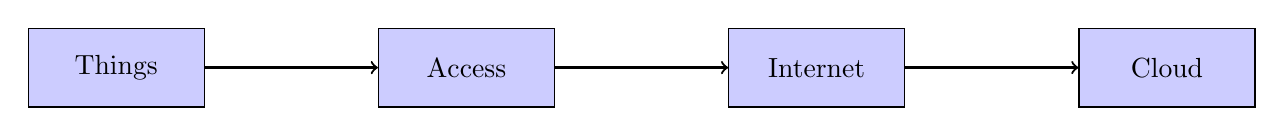
\begin{tikzpicture}[node distance=2.2cm, auto,
        block/.style={rectangle, draw, fill=blue!20, text width=2cm, text centered, minimum height=1cm}]
        
        \node[block] (things) {Things};
        \node[block, right=of things] (access) {Access};
        \node[block, right=of access] (internet) {Internet};
        \node[block, right=of internet] (cloud) {Cloud};
        
        \draw[->, thick] (things) -- (access);
        \draw[->, thick] (access) -- (internet);
        \draw[->, thick] (internet) -- (cloud);
    \end{tikzpicture}
    \end{center}
    
    \vspace{0.3cm}
    \textbf{Inside ``Things'' (embedded systems):}
    \begin{itemize}
        \item Sensing, Processing, Actuation
        \item Power, Communications, Storage
    \end{itemize}
    
    \begin{block}{This Module}
        How physical reality enters the microcontroller.
    \end{block}
\end{frame}

\begin{frame}{The Question That Matters}
    \begin{center}
        \Large
        \textit{If the cloud model is perfect but the sensor measures wrong,\\
        how ``intelligent'' is the system?}
    \end{center}
    
    \vspace{1cm}
    \begin{alertblock}{Key Insight}
        \textbf{Data quality is determined at acquisition, not in the cloud.}
        
        No amount of ML can fix bad measurements \cite{sculley2015hidden}.
    \end{alertblock}
\end{frame}

%==============================================================================
\section{What is Data Acquisition Really }
%==============================================================================

\begin{frame}{Operational Definition of DAQ}
    \textbf{Data Acquisition (DAQ) =}
    \begin{enumerate}
        \item Sample a physical signal
        \item Convert it to digital values usable by the processor
    \end{enumerate}
    
    \vspace{0.5cm}
    \textbf{The blocks:}
    \begin{center}
    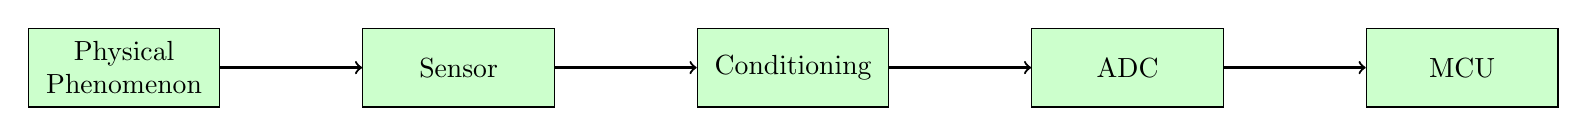
\begin{tikzpicture}[node distance=1.8cm, auto,
        block/.style={rectangle, draw, fill=green!20, text width=2.2cm, text centered, minimum height=1cm}]
        
        \node[block] (phys) {Physical Phenomenon};
        \node[block, right=of phys] (sensor) {Sensor};
        \node[block, right=of sensor] (cond) {Conditioning};
        \node[block, right=of cond] (adc) {ADC};
        \node[block, right=of adc] (mcu) {MCU};
        
        \draw[->, thick] (phys) -- (sensor);
        \draw[->, thick] (sensor) -- (cond);
        \draw[->, thick] (cond) -- (adc);
        \draw[->, thick] (adc) -- (mcu);
    \end{tikzpicture}
    \end{center}
    
    \vspace{0.3cm}
    \begin{alertblock}{Memorize This Diagram}
        Physical $\rightarrow$ Sensor $\rightarrow$ Conditioning $\rightarrow$ ADC $\rightarrow$ MCU
    \end{alertblock}
\end{frame}

\begin{frame}{Four Domains, Four Error Sources}
    \textbf{The same phenomenon exists in 4 distinct domains:}
    
    \vspace{0.5cm}
    \begin{table}
        \centering
        \begin{tabular}{clc}
            \toprule
            \textbf{\#} & \textbf{Domain} & \textbf{Error Sources} \\
            \midrule
            1 & Physical & Environmental noise, coupling \\
            2 & Electrical (analog) & Sensor nonlinearity, drift \\
            3 & Electrical (conditioned) & Amplifier noise, filtering artifacts \\
            4 & Digital & Quantization, aliasing \\
            \bottomrule
        \end{tabular}
    \end{table}
    
    \vspace{0.3cm}
    \begin{block}{Key Message}
        Errors can be introduced at \textbf{any stage}. The algorithm only sees the final result \cite{pallasareny2012sensors}.
    \end{block}
\end{frame}

%==============================================================================
\section{Sensors: What Does Measuring Mean}
%==============================================================================

\begin{frame}{Core Concepts}
    \begin{columns}[T]
        \begin{column}{0.32\textwidth}
            \textbf{Measurand}
            
            What you want to measure:
            \begin{itemize}
                \item Temperature
                \item Pressure
                \item Light
                \item pH
            \end{itemize}
        \end{column}
        \begin{column}{0.32\textwidth}
            \textbf{Sensor}
            
            Device that responds to the measurand with a signal.
        \end{column}
        \begin{column}{0.32\textwidth}
            \textbf{Transducer}
            
            Converts energy from one form to another.
            
            \vspace{0.2cm}
            \textit{(A sensor is a type of transducer)}
        \end{column}
    \end{columns}
    
    \vspace{0.5cm}
    \footnotesize
    \cite{fraden2016handbook}
\end{frame}

\begin{frame}{Classification by Energy Domain}
    \begin{table}
        \centering
        \begin{tabular}{ll}
            \toprule
            \textbf{Domain} & \textbf{Examples} \\
            \midrule
            Mechanical & Pressure, acceleration, force, displacement \\
            Thermal & Temperature, heat flux \\
            Electromagnetic & Light, RF, magnetic field \\
            Chemical & Concentration, pH, humidity \\
            \bottomrule
        \end{tabular}
    \end{table}
    
    \vspace{0.5cm}
    \footnotesize
    \cite{pallasareny2012sensors}
\end{frame}

\begin{frame}{What Makes a ``Good'' Sensor?}
    \begin{enumerate}
        \item \textbf{Sensitive} to what you want to measure
        \item \textbf{Insensitive} to everything else
        \item \textbf{Does not alter} the phenomenon being measured
    \end{enumerate}
    
    \vspace{0.5cm}
    \begin{exampleblock}{Example: Temperature Measurement}
        Measuring temperature with a large probe in a microvolume gives \textbf{false values}.
        
        \vspace{0.2cm}
        $\rightarrow$ The sensor changes the system (thermal mass).
    \end{exampleblock}
    
    \vspace{0.3cm}
    \footnotesize
    \cite{fraden2016handbook}
\end{frame}

\begin{frame}{Your Smartphone as a Sensor Lab}
    \textbf{Sensors already in your pocket:}
    
    \vspace{0.3cm}
    \begin{columns}[T]
        \begin{column}{0.48\textwidth}
            \textbf{IMU (Inertial Measurement Unit)}
            \begin{itemize}
                \item Accelerometer
                \item Gyroscope
                \item Magnetometer
            \end{itemize}
            
            \vspace{0.3cm}
            \textbf{Environmental}
            \begin{itemize}
                \item Barometer
                \item Ambient light sensor
            \end{itemize}
        \end{column}
        \begin{column}{0.48\textwidth}
            \textbf{Imaging}
            \begin{itemize}
                \item Camera (visible, IR)
                \item LiDAR (some models)
            \end{itemize}
            
            \vspace{0.3cm}
            \textbf{Biometric}
            \begin{itemize}
                \item Fingerprint
                \item Face ID sensors
            \end{itemize}
        \end{column}
    \end{columns}
    
    \vspace{0.3cm}
    \begin{block}{Connection}
        You already know these sensor: now let'sunderstand how they work.
    \end{block}
\end{frame}

%==============================================================================
\section{Signal Conditioning: The Part Nobody Wants to Design}
%==============================================================================

\begin{frame}{Why Signal Conditioning Exists}
    \begin{center}
        \Large
        \textbf{Before the ADC, the signal is almost never ready.}
    \end{center}
    
    \vspace{0.5cm}
    \textbf{Typical functions:}
    \begin{itemize}
        \item \textbf{Filtering} -- Band-limit the signal
        \item \textbf{Noise reduction} -- Improve SNR
        \item \textbf{Interference elimination} -- Reject EMI, 50/60 Hz
        \item \textbf{Amplification / Attenuation} -- Match ADC range
        \item \textbf{Impedance matching} -- Proper signal transfer
    \end{itemize}
    
    \vspace{0.3cm}
    \footnotesize
    \cite{kester2005data}
\end{frame}

\begin{frame}{Analog vs. Digital Processing}
    \begin{table}
        \centering
        \begin{tabular}{lcc}
            \toprule
            \textbf{Characteristic} & \textbf{Analog} & \textbf{Digital} \\
            \midrule
            Real-time guarantee & Yes & Depends \\
            Speed & Very fast & Clock-limited \\
            Temperature sensitivity & High & Low \\
            Tolerance sensitivity & High & None \\
            Flexibility & Fixed & Programmable \\
            Repeatability & Poor & Excellent \\
            \bottomrule
        \end{tabular}
    \end{table}
    
    \vspace{0.3cm}
    \footnotesize
    \cite{razavi2021analog}
\end{frame}

\begin{frame}{The Critical Engineering Insight}
    \begin{alertblock}{Key Rule}
        \textbf{If you don't filter before the ADC, aliasing cannot be fixed by any DSP afterwards.}
    \end{alertblock}
    
    \vspace{0.5cm}
    This connects directly to Nyquist (next section).
    
    \vspace{0.5cm}
    \begin{block}{Design Decision}
        Where you filter (analog vs. digital) directly affects:
        \begin{itemize}
            \item Power consumption
            \item Latency
            \item System complexity
        \end{itemize}
    \end{block}
\end{frame}

%==============================================================================
\section{ADC: Where Many IoT Designs Break}
%==============================================================================

\begin{frame}{Two Fundamental Operations}
    \begin{columns}[T]
        \begin{column}{0.48\textwidth}
            \textbf{1. Sampling (in time)}
            
            \vspace{0.2cm}
            Metric: Sampling frequency $f_s$
            
            \vspace{0.2cm}
            Rule: $f_s > 2 \cdot f_{max}$ (Nyquist)
        \end{column}
        \begin{column}{0.48\textwidth}
            \textbf{2. Quantization (in amplitude)}
            
            \vspace{0.2cm}
            Metric: Number of bits $N$
            
            \vspace{0.2cm}
            Result: $2^N$ discrete levels
        \end{column}
    \end{columns}
    
    \vspace{0.5cm}
    \begin{alertblock}{Irreversible}
        Both decisions are \textbf{permanent}. Information lost here cannot be recovered.
    \end{alertblock}
    
    \vspace{0.3cm}
    \footnotesize
    \cite{walden1999adc}
\end{frame}

\begin{frame}{Aliasing Explained Without Math}
    \begin{center}
        \Large
        A fast signal sampled slowly $\rightarrow$ appears as a \textbf{different, slower signal}.
    \end{center}
    
    \vspace{0.5cm}
    \textbf{Nyquist-Shannon Theorem:}
    \begin{equation}
        f_s \geq 2 \cdot f_{max}
    \end{equation}
    
    \vspace{0.3cm}
    \begin{alertblock}{Critical Rule}
        \textbf{Nyquist is not optional.}
        
        Undersampling creates false signals that are indistinguishable from real ones.
    \end{alertblock}
    
    \vspace{0.3cm}
    \footnotesize
    \cite{oppenheim1999discrete}
\end{frame}

\begin{frame}{Resolution vs. Speed: The Real Trade-off}
    \begin{table}
        \centering
        \begin{tabular}{lcc}
            \toprule
            \textbf{ADC Type} & \textbf{Resolution} & \textbf{Speed} \\
            \midrule
            Flash & 6--8 bits & $>$ 1 GSPS \\
            SAR & 12--18 bits & 1--10 MSPS \\
            Delta-Sigma ($\Sigma\Delta$) & 16--24 bits & 10--1000 SPS \\
            Dual-Slope & 12--20 bits & 10--100 SPS \\
            \bottomrule
        \end{tabular}
    \end{table}
    
    \vspace{0.3cm}
    \begin{block}{Physical Constraint}
        \textbf{No ADC is infinitely fast AND precise.}
        
        Always trade-off between: speed, resolution, power, cost \cite{kester2005data}.
    \end{block}
\end{frame}

\begin{frame}{Practical Message for IoT}
    \begin{center}
        \Large
        \textbf{In low-power IoT, you almost always sacrifice speed for energy.}
    \end{center}
    
    \vspace{0.5cm}
    \textbf{What really limits your system:}
    \begin{columns}[T]
        \begin{column}{0.48\textwidth}
            \begin{itemize}
                \item Buffer memory
                \item DMA availability
                \item Interrupt latency
            \end{itemize}
        \end{column}
        \begin{column}{0.48\textwidth}
            \begin{itemize}
                \item Power budget
                \item Real-time deadlines
                \item Processing bandwidth
            \end{itemize}
        \end{column}
    \end{columns}
    
    \vspace{0.3cm}
    \footnotesize
    \cite{wolf2012computers}
\end{frame}

%==============================================================================
\section{Sensor-MCU Interconnection}
%==============================================================================

\begin{frame}{Where is the ADC?}
    \textbf{The ADC can be located:}
    \begin{itemize}
        \item Inside the sensor (digital output sensor)
        \item Inside the MCU (internal ADC)
        \item In an external chip (dedicated ADC)
    \end{itemize}
    
    \vspace{0.5cm}
    \textbf{In all cases, data must move.}
    
    \vspace{0.3cm}
    \textbf{Classifications:}
    \begin{columns}[T]
        \begin{column}{0.32\textwidth}
            Serial vs. Parallel
        \end{column}
        \begin{column}{0.32\textwidth}
            Wired vs. Wireless
        \end{column}
        \begin{column}{0.32\textwidth}
            Synchronous vs. Async
        \end{column}
    \end{columns}
    
    \vspace{0.3cm}
    \begin{block}{Today's Reality}
        Almost everything is \textbf{serial} and \textbf{synchronous}.
    \end{block}
\end{frame}

%==============================================================================
\section{The Three Buses That Matter: SPI, I\textsuperscript{2}C, UART}
%==============================================================================

\begin{frame}{SPI -- Serial Peripheral Interface}
    \begin{columns}[T]
        \begin{column}{0.48\textwidth}
            \textbf{Characteristics:}
            \begin{itemize}
                \item Serial, Synchronous
                \item Full-duplex
                \item Master controls everything
            \end{itemize}
            
            \vspace{0.3cm}
            \textbf{Lines:}
            \begin{itemize}
                \item SCLK (clock)
                \item MOSI (master out, slave in)
                \item MISO (master in, slave out)
                \item SS/CS (one per slave)
            \end{itemize}
        \end{column}
        \begin{column}{0.48\textwidth}
            \textbf{Advantages:}
            \begin{itemize}
                \item Very fast (up to 50+ MHz)
                \item Simple protocol
                \item Ideal for high-rate sensors
            \end{itemize}
            
            \vspace{0.3cm}
            \textbf{Limitations:}
            \begin{itemize}
                \item More pins needed
                \item Scales poorly with many devices
            \end{itemize}
        \end{column}
    \end{columns}
    
    \vspace{0.3cm}
    \footnotesize
    \cite{wolf2012computers}
\end{frame}

\begin{frame}{I\textsuperscript{2}C -- Inter-Integrated Circuit}
    \begin{columns}[T]
        \begin{column}{0.48\textwidth}
            \textbf{Characteristics:}
            \begin{itemize}
                \item Serial, Synchronous
                \item Half-duplex
                \item Multi-master, multi-slave
            \end{itemize}
            
            \vspace{0.3cm}
            \textbf{Lines:}
            \begin{itemize}
                \item SDA (data)
                \item SCL (clock)
            \end{itemize}
            
            \vspace{0.3cm}
            \textbf{Protocol:}
            
            Start $\rightarrow$ Address + R/W $\rightarrow$ ACK $\rightarrow$ Data $\rightarrow$ Stop
        \end{column}
        \begin{column}{0.48\textwidth}
            \textbf{Advantages:}
            \begin{itemize}
                \item Only 2 wires
                \item Easy for many slow sensors
                \item Addressing built-in
            \end{itemize}
            
            \vspace{0.3cm}
            \textbf{Limitations:}
            \begin{itemize}
                \item More complex protocol
                \item Slower (up to 3.4 MHz)
                \item Sensitive to cable length/capacitance
            \end{itemize}
        \end{column}
    \end{columns}
    
    \vspace{0.3cm}
    \footnotesize
    \cite{pallasareny2012sensors}
\end{frame}

\begin{frame}{UART -- Universal Asynchronous Receiver-Transmitter}
    \begin{columns}[T]
        \begin{column}{0.48\textwidth}
            \textbf{Characteristics:}
            \begin{itemize}
                \item Serial, \textbf{Asynchronous}
                \item Full-duplex
                \item Point-to-point only
            \end{itemize}
            
            \vspace{0.3cm}
            \textbf{Frame format:}
            
            Idle (high) $\rightarrow$ Start bit $\rightarrow$ Data $\rightarrow$ [Parity] $\rightarrow$ Stop
        \end{column}
        \begin{column}{0.48\textwidth}
            \textbf{Advantages:}
            \begin{itemize}
                \item Ultra simple
                \item No clock line needed
                \item Ideal for debug, GPS, modules
            \end{itemize}
            
            \vspace{0.3cm}
            \textbf{Limitations:}
            \begin{itemize}
                \item Only 2 nodes
                \item Slow (typically $\leq$ 1 Mbps)
                \item Baud rate must match
            \end{itemize}
        \end{column}
    \end{columns}
    
    \vspace{0.3cm}
    \footnotesize
    \cite{white2011making}
\end{frame}

\begin{frame}{Comparison Summary}
    \begin{table}
        \centering
        \begin{tabular}{lccc}
            \toprule
            \textbf{Feature} & \textbf{SPI} & \textbf{I\textsuperscript{2}C} & \textbf{UART} \\
            \midrule
            Wires & 4+ & 2 & 2 \\
            Speed & Up to 50+ MHz & Up to 3.4 MHz & Up to 1 Mbps \\
            Topology & Point-to-point & Multi-drop bus & Point-to-point \\
            Synchronization & Clock & Clock & Baud rate \\
            Duplex & Full & Half & Full \\
            Complexity & Low & Medium & Very low \\
            \bottomrule
        \end{tabular}
    \end{table}
    
    \vspace{0.3cm}
    \footnotesize
    \cite{wolf2012computers}
\end{frame}

%==============================================================================
\section{Final Activity: Choose Your Bus}
%==============================================================================

\begin{frame}{Scenario A}
    \textbf{Setup:}
    \begin{itemize}
        \item 1 MCU + 5 slow sensors on the same board
        \item Minimum wiring required
    \end{itemize}
    
    \vspace{0.5cm}
    \pause
    \begin{block}{Answer: I\textsuperscript{2}C}
        \begin{itemize}
            \item Only 2 wires for all 5 sensors
            \item Each sensor has unique address
            \item Speed is sufficient for slow sensors
        \end{itemize}
    \end{block}
    
    \vspace{0.3cm}
    \textbf{Justify by:} number of devices, wiring complexity, speed requirements
\end{frame}

\begin{frame}{Scenario B}
    \textbf{Setup:}
    \begin{itemize}
        \item IMU at 10 kHz for motion control
        \item Real-time performance critical
    \end{itemize}
    
    \vspace{0.5cm}
    \pause
    \begin{block}{Answer: SPI}
        \begin{itemize}
            \item High speed required (10 kHz $\times$ 6 axes $\times$ 16 bits)
            \item Full-duplex for fast read cycles
            \item Single device, so pin count is acceptable
        \end{itemize}
    \end{block}
    
    \vspace{0.3cm}
    \textbf{Justify by:} speed, real-time requirements, data throughput
\end{frame}

\begin{frame}{Scenario C}
    \textbf{Setup:}
    \begin{itemize}
        \item MCU + external module
        \item Only text console needed (debug/logging)
    \end{itemize}
    
    \vspace{0.5cm}
    \pause
    \begin{block}{Answer: UART}
        \begin{itemize}
            \item Simplest protocol
            \item Human-readable text
            \item No addressing needed (point-to-point)
        \end{itemize}
    \end{block}
    
    \vspace{0.3cm}
    \textbf{Justify by:} simplicity, use case, legacy compatibility
\end{frame}

\begin{frame}{Decision Criteria Summary}
    \textbf{When choosing a bus, consider:}
    
    \vspace{0.5cm}
    \begin{table}
        \centering
        \begin{tabular}{ll}
            \toprule
            \textbf{Criterion} & \textbf{Question to Ask} \\
            \midrule
            Speed & What data rate do I need? \\
            Device count & How many peripherals? \\
            Complexity & How much protocol overhead is acceptable? \\
            Power & What is my energy budget? \\
            Pins & How many GPIOs can I spare? \\
            \bottomrule
        \end{tabular}
    \end{table}
    
    \vspace{0.3cm}
    \begin{block}{Engineering Mindset}
        There is no ``best'' bus but the \textbf{right bus for your requirements}.
    \end{block}
\end{frame}

%==============================================================================
% Summary
%==============================================================================

\begin{frame}{Module Summary}
    \textbf{Key Takeaways:}
    
    \vspace{0.3cm}
    \begin{enumerate}
        \item \textbf{Pipeline:} Physical $\rightarrow$ Sensor $\rightarrow$ Conditioning $\rightarrow$ ADC $\rightarrow$ MCU
        \item \textbf{Sensors:} Measurand $\neq$ Sensor $\neq$ Transducer
        \item \textbf{Conditioning:} Filter \textit{before} ADC or aliasing is permanent
        \item \textbf{ADC:} Nyquist ($f_s > 2f_{max}$), resolution vs. speed trade-off
        \item \textbf{Buses:} SPI (fast), I\textsuperscript{2}C (many devices), UART (simple)
    \end{enumerate}
    
    \vspace{0.3cm}
    \begin{alertblock}{Remember}
        Data quality is determined at acquisition. No cloud ML can fix bad measurements.
    \end{alertblock}
\end{frame}

%==============================================================================
% References
%==============================================================================

\begin{frame}[allowframebreaks]{References}
    \printbibliography
\end{frame}

\end{document}
